\section{Numerical Tests}

The setup is shown in Fig. \ref{fg:config}, where the heavy (liquid) and light (gas) phases are represented with gray and white colors respectively. The distance $h$ between the cylinder top and the undisturbed free surface is taken as the measure of the cylinder submergence. Uniform inflow velocity with module $U$ is imposed on the inlet. The chosen Froude number based on the diameter of the cylinder $d$ is
\begin{equation}
 Fr = \frac{U}{\sqrt{gd}}
\label{eq:froude}
\end{equation}
where $g$ is the gravity acceleration. Also, the Reynolds number is calculated based on $U$ and $d$ as characteristic velocities and length respectively, being
\begin{equation}
 Re = \frac{U d}{\mu_l}
\label{eq:reynolds}
\end{equation}
with $\mu_l$ the dynamic viscosity of the heavier phase.

\begin{figure}[ht]
  \centering
  %%----primera subfigura----
  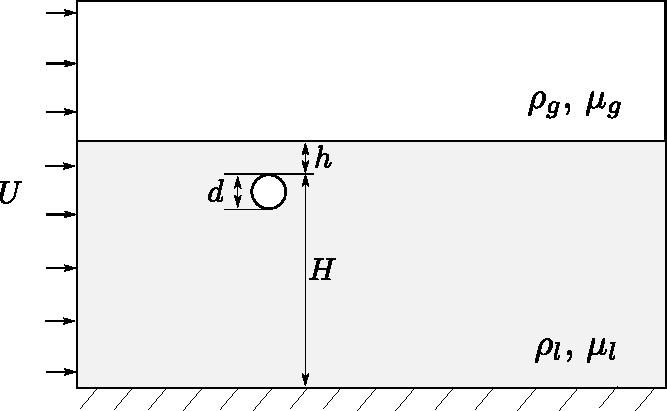
\includegraphics[width=0.4\textwidth]{images_10thspheric/config.pdf}
  \caption{Case configuration, initial and boundary conditions.}
  \label{fg:config}
\end{figure}

In the reference work of Reichl et.al \cite{Reichl05}, densities and viscosities ratios are established in $\rho_l/\rho_g = \mu_l/\mu_g=100$ in order to avoid convergence problems. PFEM-2 method does not suffer from these drawbacks, allowing more realistic water-air ratios. However, the original ratios are employed to guarantee same simulation conditions. Regarding to boundary conditions, an uniform flow $U$ is imposed at the inlet, leaving free the outlet velocity. The floor of the channel and the cylinder surface are considered no-slip, and atmosphere condition is set at the top of the geometry.

Flow conditions are inspirated in the work of Bouscasse \cite{Bouscasse14} which investigates the flow behavior employing a range of Froude numbers for a fixed submergence ($h/d=0.55$ ratio) and a fixed Reynolds number of $Re=180$. The mentioned reference uses SPH as numerical method allowing to treat larger fragmentation of the free surface, compared to FLUENT-VOF technique used by Reichl and colleagues. The PFEM-2 method employed in the current work, since its particle nature, is also able to treat large deformations and breakups.

A summary of computed forces can be seen in Fig. \ref{fg:CdCl}. The drag coefficient slightly diminishes as Froude number increases. A maximum lift (in absolute value) is found for $Fr = 0.8$, and then a gentle monotonic reduction for the largest Froude number cases occurs. Good agreement with the reference work can be observed.

\begin{figure}[ht]
  \centering
  %%----primera subfigura----
  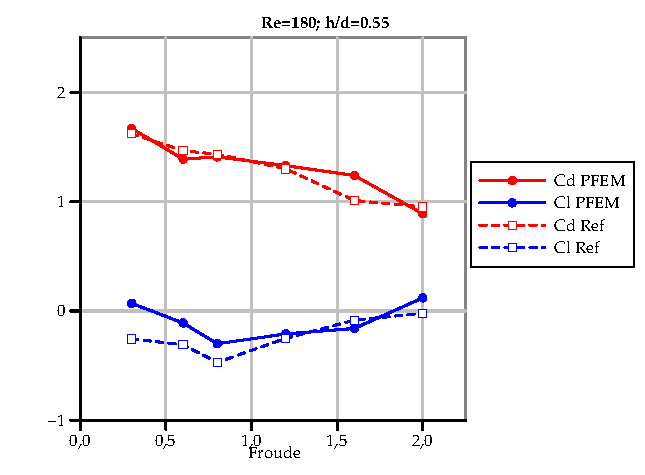
\includegraphics[width=0.5\textwidth]{images_10thspheric/CdCl_cylinder_surface.pdf}
  \caption{Drag and Lift coefficients calculated with PFEM-2 compared with the reference work of Bouscasse \cite{Bouscasse14}.}
  \label{fg:CdCl}
\end{figure}
